%! LuaLaTeX 文書
\documentclass[unicode,colorlinks]{beamer}
\usetheme{metropolis}
\usefonttheme{professionalfonts}

\hypersetup{linkcolor=blue,urlcolor=teal}

\usepackage{luatexja}
\ltjsetparameter{jacharrange={-2,-3,-8}}
\usepackage[no-math,match,deluxe]{luatexja-preset}

\usepackage{graphicx,xcolor}
\usepackage{pxrubrica}
\usepackage{tcolorbox}
\usepackage{bxwareki}

\usepackage{tikz}
\usetikzlibrary{plotmarks}

\usepackage{bxokumacro}
\usepackage{keystroke}

\usepackage[T1]{fontenc}
\usepackage{amsmath,mathtools,amssymb,mathrsfs,rsfso,mleftright}
\usepackage[math]{kurier}
\usepackage[euler-digits]{eulervm}
\usepackage[scaled]{beramono}
\allowdisplaybreaks[4]

%%%%%%%%%% 商用フォントを用いているので、自分でタイプセットする場合は適当に以下を変えてください
\setmainfont[
	Ligatures=TeX,
	BoldFont=FOT-RodinNTLGPro-EB,
	ItalicFont=FOT-RodinNTLGPro-EB,
]{FOT-RodinNTLGPro-B}
\setsansfont[
	Ligatures=TeX,
	BoldFont=FOT-RodinNTLGPro-EB,
	ItalicFont=FOT-RodinNTLGPro-EB,
]{FOT-RodinNTLGPro-B}
\setmainjfont[
	Ligatures=TeX,
	CharacterWidth=Proportional,
	JFM=prop,
	BoldFont=FOT-RodinNTLGPro-EB,
	ItalicFont=FOT-RodinNTLGPro-EB,
]{FOT-RodinNTLGPro-B}
\setsansjfont[
	Ligatures=TeX,
	CharacterWidth=Proportional,
	JFM=prop,
	BoldFont=FOT-RodinNTLGPro-EB,
	ItalicFont=FOT-RodinNTLGPro-EB,
]{FOT-RodinNTLGPro-B}
\setmonofont[
	Ligatures=TeX
]{DejaVu Sans Mono}
\setmonojfont[
	Ligatures=TeX,
]{NotoSansMonoCJKjp-Regular}

%%%%%%%%%% 以下は自前コマンド

\newcommand{\centeralign}[1]{\rule{0pt}{0pt}\hfill#1\hfill\rule{0pt}{0pt}}
\newcommand{\Unit}[1]{\,\mathrm{#1}}

\setlength{\parskip}{2ex}

\title{大気放射の基礎\\--Liou著 藤枝・深堀訳 (2014) の講読--}
\author{北海道大学理学部 人見祥磨}
\date{\warekitoday}

\begin{document}
\maketitle

\begin{frame}{目次}
	\tableofcontents
\end{frame}

\section{動機}

\begin{frame}{動機}
	\begin{itemize}
		\item 惑星大気の熱輸送について興味があった
		\item 惑星大気について、自転周期や地軸の傾きによって、
			どのように熱輸送が変化するかシミュレーションしたい
		\item そのために、大気の温度分布を知りたい
		\item 放射に関する基本的な事項の知識の確認
		\item 放射に関して、観測なども含めて、基礎事項を解説している Liou の教科書を
			読むことにした
			\begin{itemize}
				\item 大気放射学 {\scriptsize---衛星リモートセンシングと気候問題へのアプローチ---}\\
					K.N.Liou(著) 藤枝 鋼、深堀 正志(翻訳)\\
					共立出版 \textbf{(2014)} 672ページ
			\end{itemize}
	\end{itemize}
\end{frame}

\begin{frame}
	\section{基本的な放射量}

	放射が進行することで、放射は相互作用により増減する。これを記述する
	\textbf{放射伝達方程式}を導くことが目的である。

	そのために、放射量を表すための物理量の定義について確認する。
\end{frame}

\begin{frame}{基本的な放射量}
	\begin{description}
		\item[単色の放射強度 $I_\lambda$]\leavevmode\\
			面積 $dA$ を横切り、$dA$ の法線からなす角 $\theta$ の方向にある
			微小立体角 $d\Omega$ から入射する、ある波長区間 $\lambda$ 〜
			$\lambda+d\lambda$ における、微小時間 $dt$ の間の微小放射エネルギー量
			$dE_\lambda$
			\[dE_\lambda=I_\lambda\cos[\theta]\,dA\,d\Omega\,d\lambda\,dt\]
			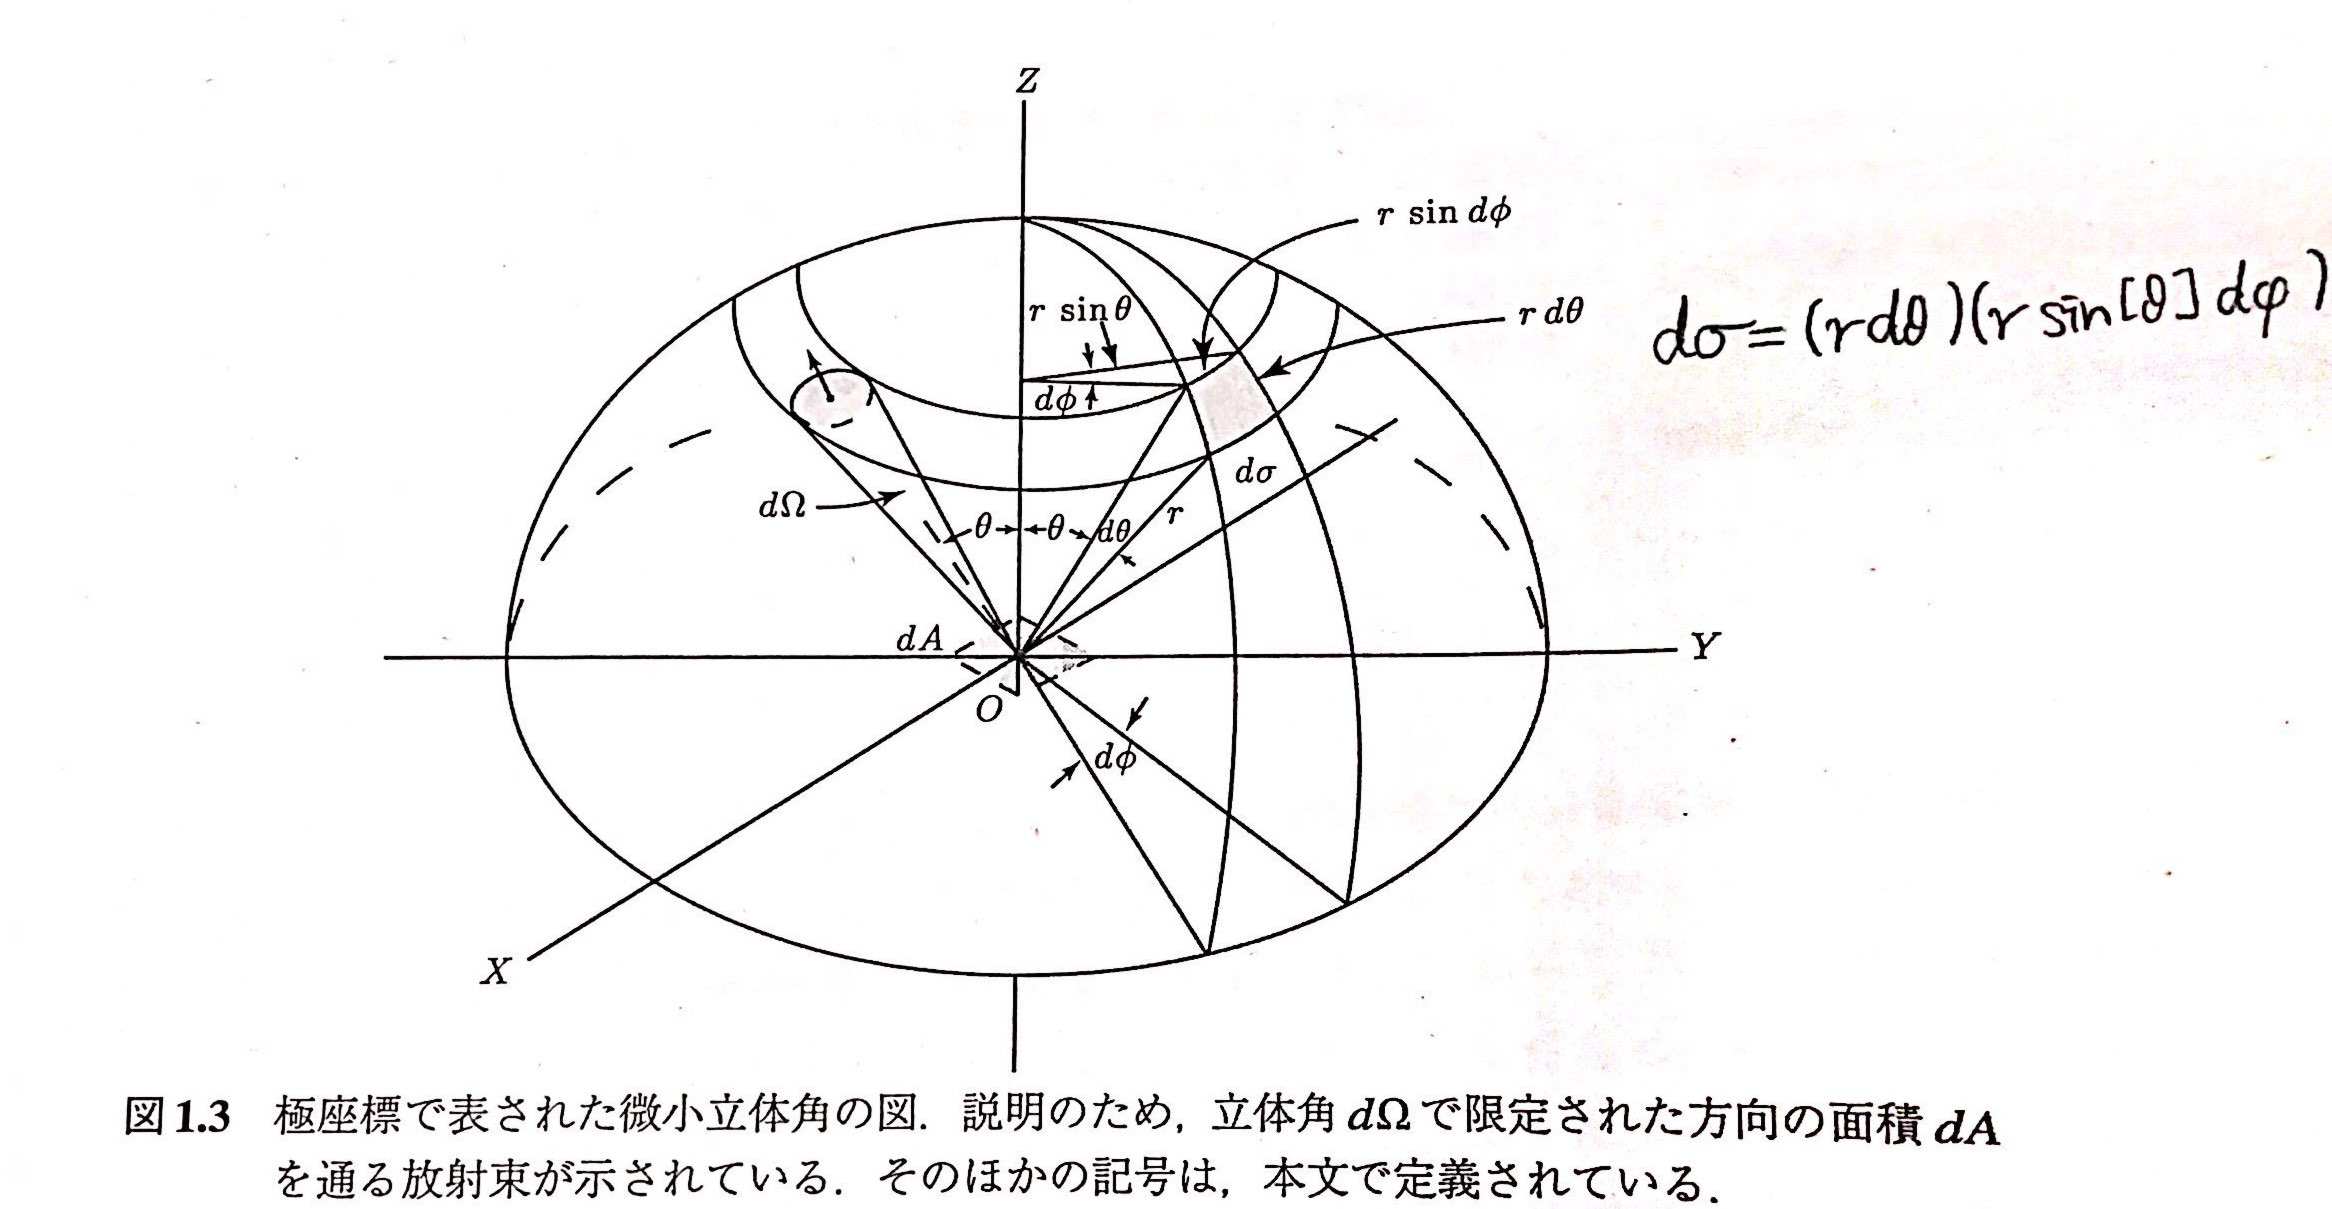
\includegraphics[width=\linewidth]{eq.jpg}
	\end{description}
\end{frame}

\begin{frame}{基本的な放射量}
	\begin{description}
		\item[単色の放射フラックス密度 $F_\lambda$]\leavevmode\\
			単色の放射輝度を、半球の全立体角にわたって積分したものの、法線成分
			\[F_\lambda=\int_\Omega I_\lambda\cos[\theta]\,d\Omega\]
		\item[全放射フラックス密度 $F$]\leavevmode\\
			単色の放射フラックス密度を、波長全体で積分
			\[F=\int^\infty_0 F_\lambda\,d\lambda\]
		\item[全放射フラックス $f$]\leavevmode\\
			全放射フラックス密度を、面全体で積分
			\[f=\int_AF\,dA\]
	\end{description}
\end{frame}

\begin{frame}
	\section{散乱と吸収の概念}
	放射は、散乱や吸収の過程を経て、強度が変化する。

	このことは、放射伝達方程式に記述されるが、実際にどのような現象が
	発生しているか確認する。
\end{frame}

\begin{frame}{散乱と吸収の概念}
	\begin{description}
		\item[散乱] 入射波と衝突した粒子が、入射した電磁波のエネルギーを、あらゆる方向に
			再放射する過程。すべての波長で発生し、粒子の大きさが影響する。
			\begin{description}
				\item[独立散乱] 粒子が少ないとき、個々の粒子が全く同じように散乱する。
				\item[多重散乱] 粒子が多量にあるとき、散乱が繰り返される。\\
					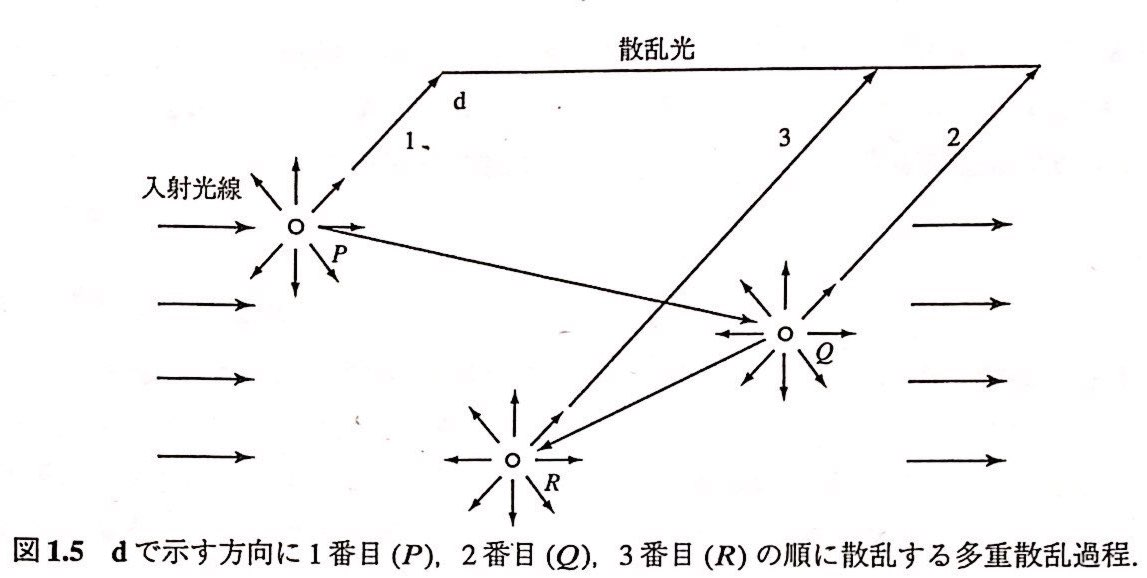
\includegraphics[width=\linewidth]{mscatter.jpg}
			\end{description}
		%\item[吸収] 吸収されたエネルギーは、もはや光として存在しない。
	\end{description}
\end{frame}

\begin{frame}{散乱の種類}
	散乱にはサイズパラメーター $x=2\pi a/\lambda$ ($a$ は粒径)が影響

	\centeralign{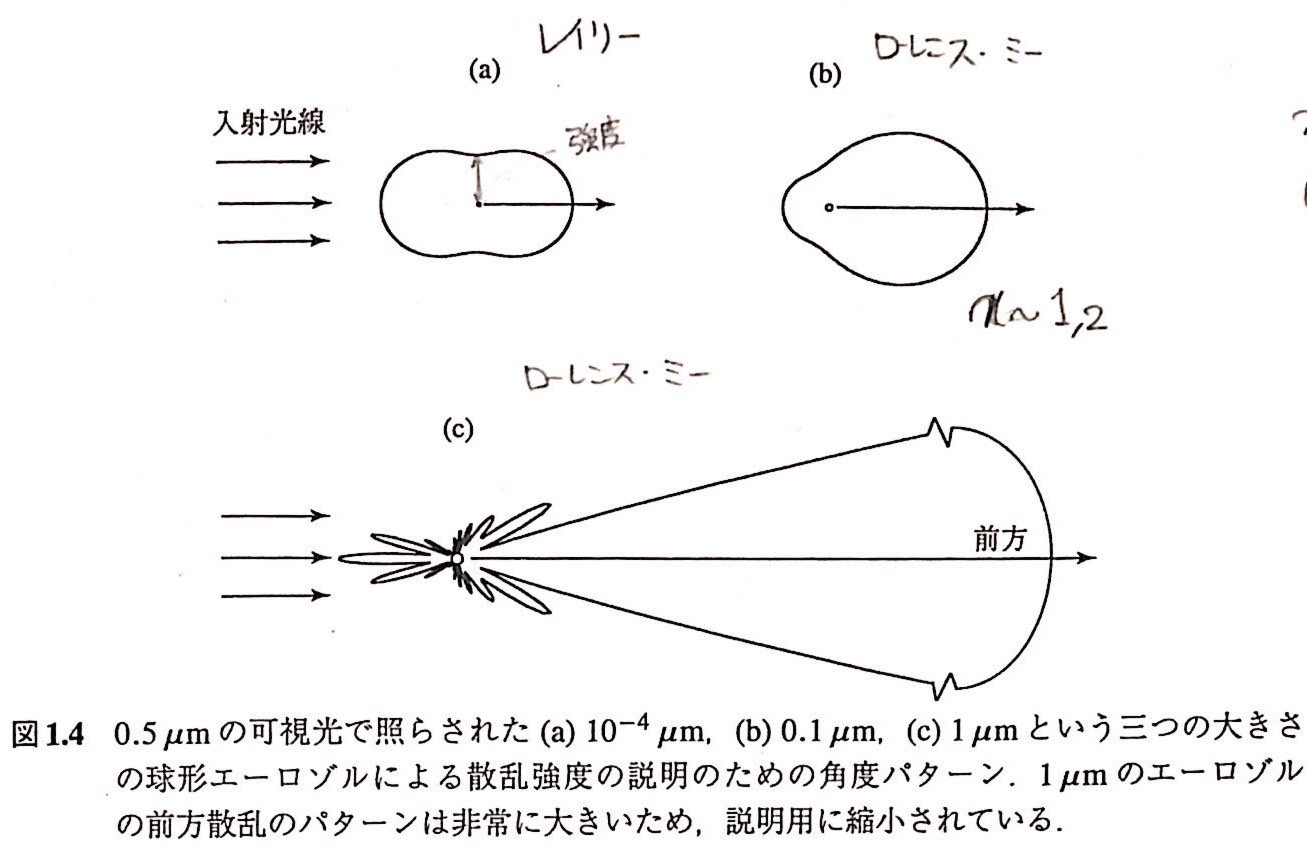
\includegraphics[width=0.8\textwidth]{scatter.jpg}}
\end{frame}

%\begin{frame}{吸収係数}
	%\begin{description}
		%\item[断面積] 粒子によってもとの光線から取り去られたエネルギー量を
			%表すために用いられる用語。幾何学的な面積に類する。単位は
			%$\Unit{cm^2}$ に換算。
		%\item[質量消散断面積] 断面積が単位質量に関連するとき、断面積は
			%$\Unit{cm^2\,g^{-1}}$ に換算。
	%\end{description}
%\end{frame}

\begin{frame}
	\section{黒体放射の法則}

	黒体とは吸収のない理想的な物体である。
	放射を考える上で、最も基本的な物体として黒体を考える。

	黒体の放射を支配する 4 つの法則について述べる。
\end{frame}

%\begin{frame}{黒体}
	%\begin{description}
		%\item[黒体とは] 吸収が完全である素材\\

	%\end{description}

	%以下、黒体放射を支配する 4 つの法則について述べる

	%\centeralign{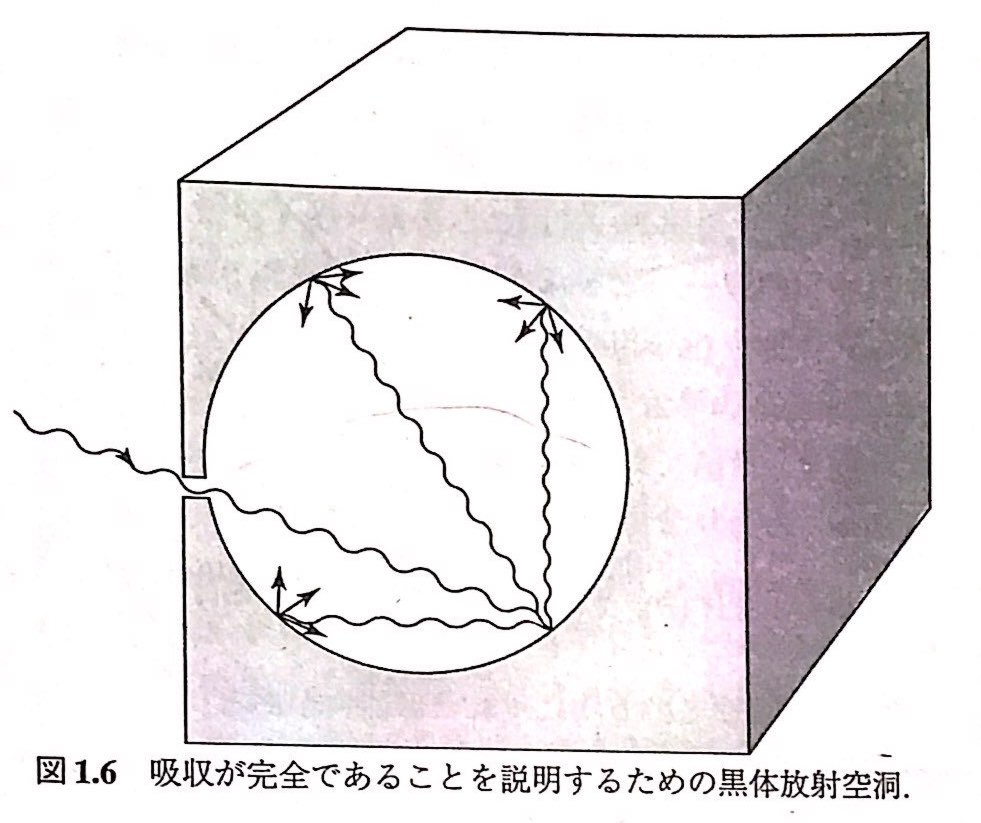
\includegraphics[width=0.5\textwidth]{black.jpg}}

	%細い穴からフラックスが入射し、空洞内に閉じ込められ、全てが吸収されるまで内部反射が
	%繰り返される
%\end{frame}

\begin{frame}{プランクの法則}
	振動子が持つエネルギーは $E=nh\tilde{\nu}$ に量子化されると仮定する

	プランク関数: $\displaystyle B_{\tilde{\nu}}[T]=\frac{2h\tilde{\nu}^3}{c^2(\exp[h\tilde{\nu}/k_\mathrm{B}T]-1)}$\\
	{\scriptsize ($\tilde{\nu}$: 周波数、$h$: プランク定数、$k_\mathrm{B}$: ボルツマン定数、
	$c$: 光速、$T$: 絶対温度)}

	射出された単色の放射強度を、周波数と射出する物質の温度に関連付ける

	波長$\lambda$に関するプランク関数:
	\[B_\lambda[T]=\frac{2hc^2}{\lambda^5(\exp[hc/k_\mathrm{B}\lambda T]-1}=
		\frac{C_1\lambda^{-5}}{\pi(\exp[C_2/\lambda T]-1)}\]
	{\scriptsize ($C_1=2\pi hc^2, C_2=hc/k_\mathrm{B}$)}
\end{frame}

\begin{frame}{プランクの法則}
	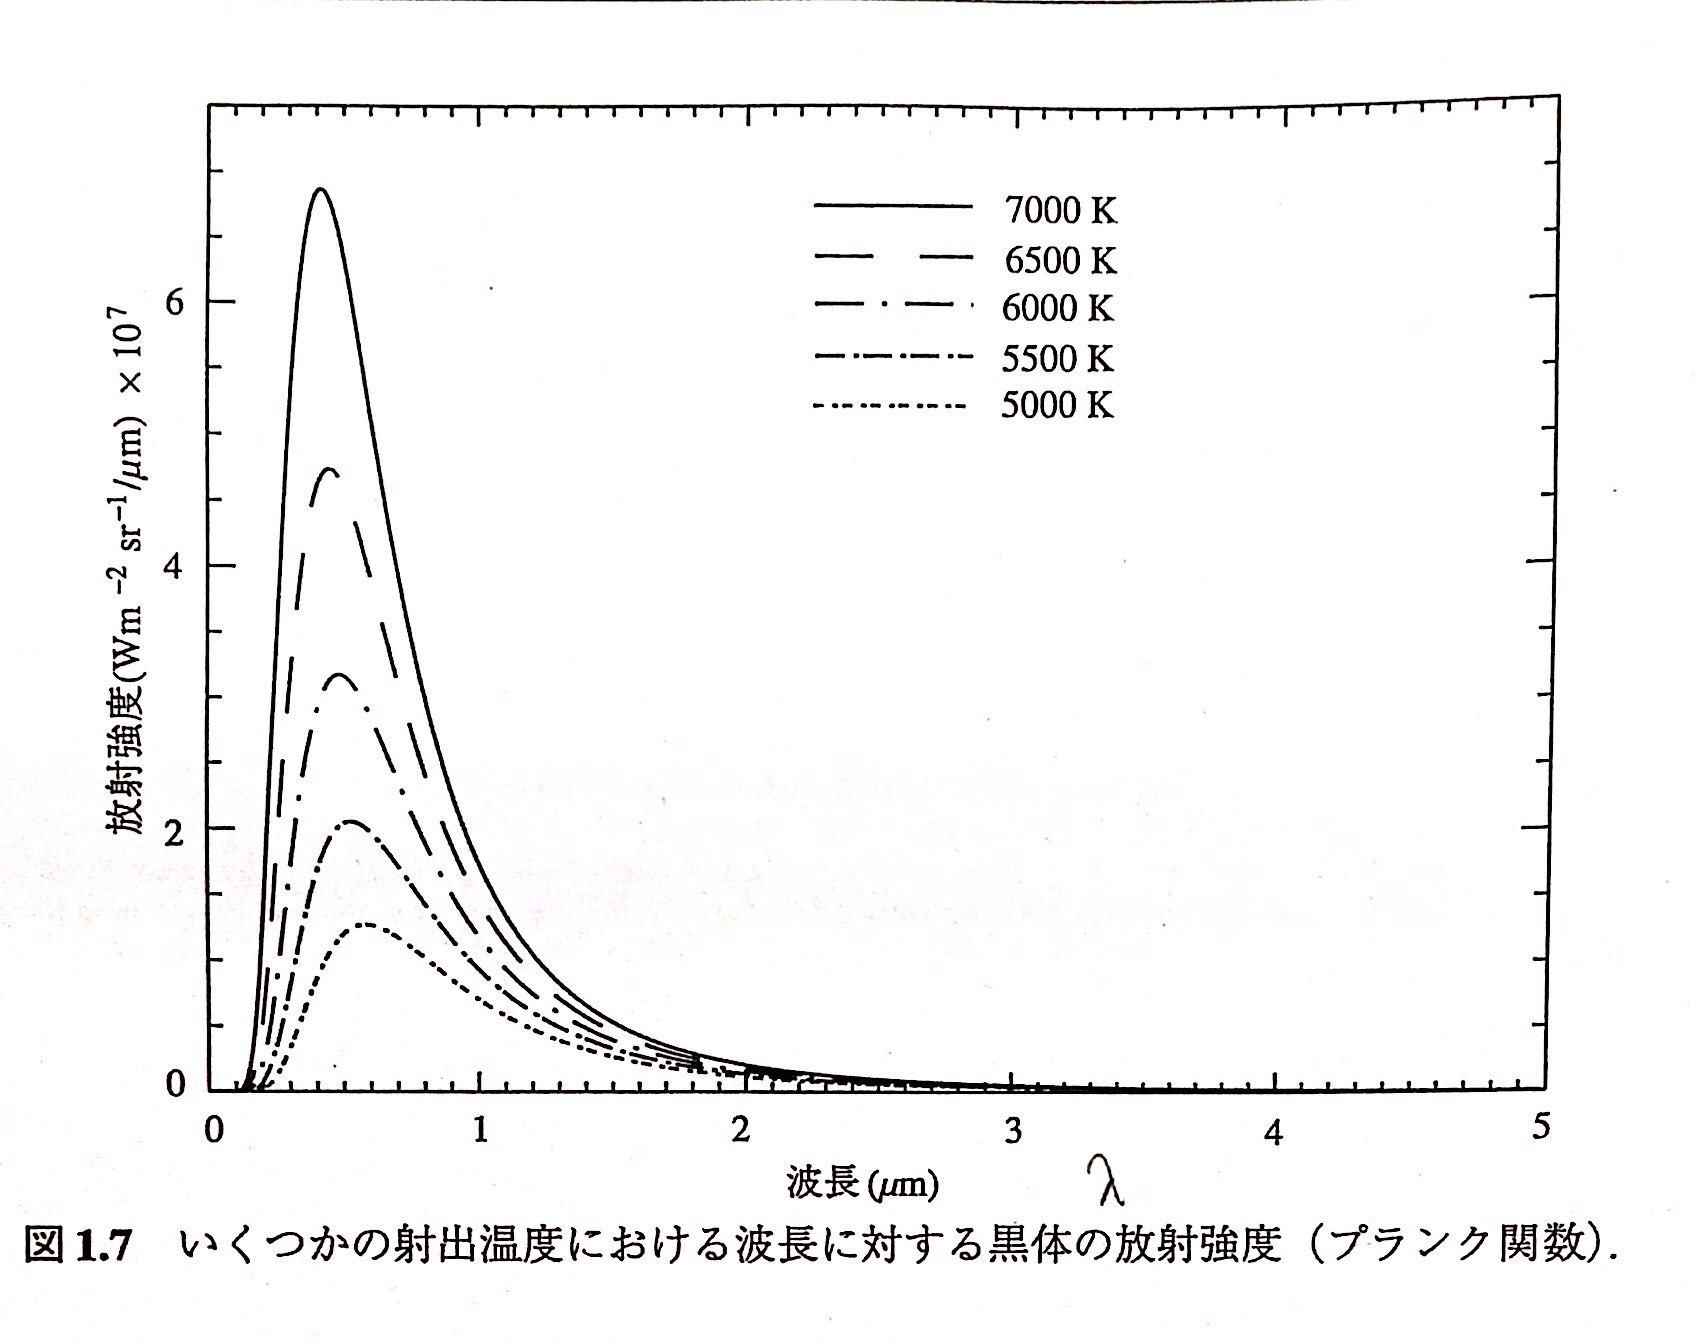
\includegraphics[width=\textwidth]{planck.jpg}
\end{frame}

\begin{frame}{ステファン・ボルツマンの法則}
	黒体の全放射強度: プランク関数を波長全体で積分

	\[B[T]=\int^\infty_0 B_\lambda[T]\,d\lambda=bT^4, \qquad b=\frac{2\pi^4k_\mathrm{B}^4}{15c^2h^3}\]

	等方な黒体によって放射される放射フラックス密度: \[F=\pi B[T]=\sigma T^4\]
	$\sigma=5.67\times10^{-8}\Unit{J\,m{-2}\,s^{-1}\,k_\mathrm{B}^{-4}}$; ステファン・ボルツマン定数

	広い波長域での赤外放射伝達の解析の基礎となる
\end{frame}

\begin{frame}{ウィーンの変位則}
	黒体放射の最大放射強度の波長が、温度に反比例する

	\[\frac{\partial B_\lambda[T]}{\partial\lambda}=0\quad\text{これを解くと}\quad\lambda_m=\frac{a}{T}\]
	($a=2.897\times10^{-3}\Unit{m\,K}$; ウィーンの変位定数)
\end{frame}

\begin{frame}{キルヒホッフの法則}
	以下の条件を満たしているとき、射出と吸収が等しくなる

	\begin{itemize}
		\item 一様な温度
		\item 等方性放射
		\item 熱力学的平衡
	\end{itemize}

	中間圏よりも高度が低い、局所的に限られた空間では、
	エネルギー遷移が分子の衝突によって支配される範囲内で、精度良く成り立つと考えて良い
\end{frame}

%\section{吸収線の形成と線形}

%\begin{frame}{吸収線の形成}
%\end{frame}

%\begin{frame}{線の広がり}
%\end{frame}

\begin{frame}
	\section{放射伝達の基礎}
	ある方向に進む放射が、吸収や散乱などの相互作用で、どのように増減するか
	記述するのが、放射伝達方程式である。

	放射伝達方程式を導き、特定の状況での放射伝達方程式の解を求める。
\end{frame}

\begin{frame}{放射伝達方程式}
	放射伝達強度 $I_\lambda^\mathrm{d}$ が、放射の伝搬方向に厚さ $ds$ で密度 $\rho$ の媒質を横切った後に、
	$I_\lambda^\mathrm{d}+dI_\lambda^\mathrm{d}$ になるとする
	\[dI_\lambda^\mathrm{d}=-k_\lambda\rho i_\lambda\,ds\]
	$k_\lambda$ は質量消散断面積と呼ばれる

	射出と多重散乱による放射強度の増加が以下で与えられるように、
	放射源係数 $j_\lambda$ を定義する
	\[dI_\lambda^\mathrm{s}=j_\lambda\rho\,ds\]
\end{frame}

\begin{frame}{放射伝達方程式}
	ふたつの式を関連付けて、
	\[dI_\lambda=dI_\lambda^\mathrm{d}+dI_\lambda^\mathrm{s}=-k_\lambda\rho I_\lambda\,ds+j_\lambda\rho\,ds\]

	放射源関数 $J_\lambda\equiv j_\lambda/k_\lambda$ を導入すると、
	\[\frac{dI_\lambda}{k_\lambda\rho\,ds}=-I_\lambda+J_\lambda\quad\text{……放射伝達方程式}\]
\end{frame}

\begin{frame}{ビーアー・ブーゲー・ランバートの法則}
	大気系からの射出の寄与を無視できる
	\[\frac{dI_\lambda}{k_\lambda\rho\,ds}=-I_\lambda\]

	積分すると
	\[I_\lambda[s_1]=I_\lambda[0]\exp[-k_\lambda u],\qquad u=\int^{s_1}_0\rho\,ds\quad\text{(光路長)}\]

	一様に消散する媒質を横切る放射強度の低下が、質量消散断面積と
	光路長の積の指数関数に従う
\end{frame}

\begin{frame}{シュワルツシルトの方程式}
	地球と大気から射出される熱赤外放射伝達\\
	放射源関数はプランク関数で与えられる

	放射伝達方程式: シュワルツシルトの式
	\[\frac{dI_\lambda}{k_\lambda\rho\,ds}=-I_\lambda+B_\lambda[T]\]

	シュワルツシルトの式の解:
	\[I_\lambda[s_1]=I_\lambda[0]\exp\bigl[-\tau_\lambda[s_1,0]\bigr]+
		\int^{s_1}_{0}B_\lambda\bigl[T[s]\bigr]\exp\bigl[-\tau_\lambda[s_1,s]\bigr]k_\lambda\rho\,ds\]
	\[\tau_\lambda[s_1,s]=\int^{s_1}_s k_\lambda\rho\,ds\qquad\text{($s$ と $s_1$ の間の光学的厚さ)}\]
\end{frame}

%\begin{frame}{平行平面大気の放射伝達方程式}
%\end{frame}

\section{まとめ}

\begin{frame}{まとめ・今後の展望}
	\begin{itemize}
		\item 基礎方程式の概念がわかった
		\item 特定の状況(大気系からの射出を無視できる場合や、シュワルツシルトの方程式)
			での、放射伝達方程式の解法を学んだ
		\item 放射伝達方程式から計算できるもの
			\begin{itemize}
				\item 放射伝達方程式から吸収の鉛直分布を求めることができる
				\item その結果、気温の鉛直分布がわかるようになる
			\end{itemize}
		\item 実際に応用する方法がわかっていないので、第 8 章を読み進めているところ
	\end{itemize}
\end{frame}
\end{document}
